\section{Mixed Practice}

\subsection{Warm Ups}
These are good problems for reinforcing the vocabulary and foundational concepts of this chapter.

\begin{exercise}{\Coffeecup \Coffeecup }

\begin{enumerate}[label=\alph*.)] 

\item  Graph the polar function $r(\theta)=4\sec(\theta)$ by picking a spread of $\theta$ values and making an input-output table.
\solushun{\begin{tabular}{c|c|c|c|c}
$\theta$ & 0 & $ \pi/6$ & $\pi/4$ & $\pi/3$   \\ 
$r(\theta)$ & 4 & $8/\sqrt{3}$ & $8/\sqrt{2}$ & 8  \\
\end{tabular}
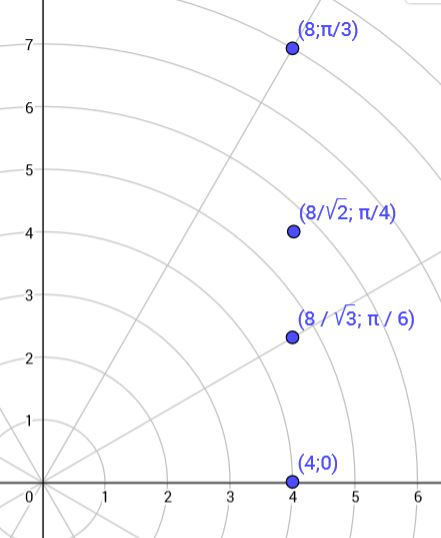
\includegraphics[scale=0.35]{ChapterCalcIII/Figures/polarpic1.jpg}
 }{0in}

\item Convert to cartesian coordinates to show that the graph is in fact just a line!
\solushun{$r=4\sec{\theta} \Longrightarrow r \cos{\theta} = 4 \Longrightarrow  x=4$ is a vertical line.
\\ }{0in}

\item Sketch the polar region whose area corresponds to the following integral: $$A=\int_{\theta=0}^{\theta=\pi/4}\frac{1}{2}\left( 4\sec(\theta)\right)^2 \mathtt{d}\theta $$
\solushun{Since this is the calculation for the area under the curve $4 \sec{\theta}$ in polar form, we have the region:
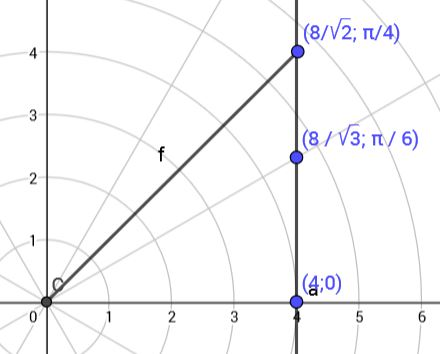
\includegraphics[scale=0.35]{ChapterCalcIII/Figures/polarpic2.jpg}
\\ }{0in}

\item What shape is the region sketched in c)?  Find the area by basic geometry. 
\solushun{It is an isosceles triangle with hypotenuse $4\sqrt{2}$ and sides 4 so $A = \frac{1}{2} b \cdot h = \frac{1}{2} 4 \cdot 4 = 8$ so we get 
\\ }{0in}

\item Find the area by computing the integral.  Verify your answers match.  
\solushun{$A = \int_0^{\pi/4}{\frac{1}{2} (4\sec{\theta})^2~d\theta} = \int_0^{\pi/4}{\frac{1}{2} (16\sec^2{\theta})~d\theta}= 8 \tan{\theta} \Biggr|_0^{\pi/4} = 8 \left( \tan {\pi/4} - \tan{0} \right) = 8 \cdot 1 - 8 \cdot 0 = 8$  They are the same. 
\\ }{0in}
\end{enumerate}

\AnswerKeyEntry{a.~~ $r(0) = 4,~~r(\pi/6) = 8/\sqrt{3},~~r(\pi/4) =8/\sqrt{2}=4\sqrt{2},~~r(\pi/3)= 8 $ 
b.~~ $r=4\sec{\theta} \Longrightarrow r \cos{\theta} = 4 \Longrightarrow  x=4$ is a vertical line. 
c.~~
d.~~It is an isosceles triangle with hypotenuse $4\sqrt{2}$ and sides 4 $A=8$
e.~~$A=8$ They are the same.
}
\end{exercise}


\begin{exercise}{\Coffeecup \Coffeecup }
Consider the parameterization $$ \{ (4t-1,6t): t\in [0,2] \}$$
That is, $x(t)=4t-1$ and $y(t)=6t$ as $t$ roams from 0 to 2.
\begin{enumerate}[label=\alph*.)]
\item Describe the shape of this parametric curve.
\solushun{ It is a line segment that lies on the line $\frac{x-1}{4} = t = \frac{y}{6} \leftrightarrow y = \frac{3}{2} x - \frac{3}{2} $ between $(-1,0)$ and $(7,12)$
\\ }{0in}

\item What is the slope of the tangent line to the parametric curve at $t=1$?  
\solushun{ $\frac{dy}{dx} = \frac{dy/dt}{dx/dt} = \frac{6}{4} = \frac{3}{2}$ which is the slope of the line.
\\ }{0in}

\item Use the parametric arc length formula to compute the length of the parameterized curve from part a). 
\solushun{ $L = \int_{t=0}^{t=2}{\sqrt{(x'(t))^2+(y'(t))^2}~dt}=\int_0^2{\sqrt{4^2+6^2}~dt} = \int_0^2{\sqrt{52}~dt} =2\sqrt{13} t \Biggr|_0^2 = 4\sqrt{13}$ 
\\ }{0in}
\end{enumerate}
\AnswerKeyEntry{a.)~~ It is a line segment that lies on the line $\frac{x-1}{4} = t = \frac{y}{6} \leftrightarrow y = \frac{3}{2} x - \frac{3}{2} $ between $(-1,0)$ and $(7,12)$ \newline
b.)~~$\frac{3}{2}$ \newline
c.)~~ $4\sqrt{13}$}
\end{exercise}



\subsection{Sample Test Problems}
\begin{exercise}{\Coffeecup \Coffeecup \Coffeecup }
State the power series definitions for hyperbolic sine and cosine:

\begin{itemize}
\item $\cosh(t)=$
\item $\sinh(t)=$
\end{itemize}
\solushun{$\cosh{t} = 1+\frac{t^2}{2!} + \frac{t^4}{4!}+\frac{t^6}{6!} + \cdots $\\
$\sinh{t} = t + \frac{t^3}{3!} + \frac{t^5}{5!}+ \cdots $
\\ }{0in}
\begin{enumerate}[label=\alph*.)] 

\item Use the power series for hyperbolic sine to compute its derivative.
\solushun{$\frac{d ~\sinh(t)}{dt} = 1+\frac{t^2}{2!}+\frac{t^4}{4!} + \cdots =\cosh(t)$
\\ }{0in}

\item Use the power series for hyperbolic cosine to compute its derivative.
\solushun{$\frac{d ~\cosh(t)}{dt} = t+\frac{t^3}{3!}+\frac{t^5}{5!} + \cdots =\sinh(t)$
\\ }{0in}

\item Consider the parametric curve $$\lbrace (\cosh(t),\sinh(t)): t\in \mathbb{R} \rbrace $$ 

Verify out to degree six that this parametric curve also satisfies the cartesian equation for the same hyperbola given by: $$x^2-y^2=1 $$

by plugging the power series formulas for our hyperbolic trig functions in for $x$ and $y$.
\solushun{$ \cosh^2{t}- \sinh^2{t} = \left(1+\frac{t^2}{2!} + \frac{t^4}{4!}+\frac{t^6}{6!} + \cdots \right)^2 - \left(t + \frac{t^3}{3!} + \frac{t^5}{5!}+ \cdots \right)^2 = \left( 1 + \frac{t^2}{2!}+\frac{t^2}{2!} + \frac{t^4}{4!} + \frac{t^4}{4!} + \frac{t^4}{2!2!} + \frac{t^6}{6!}+\frac{t^6}{6!} + \frac{t^6}{4!2!}+\frac{t^6}{4!2!} + \cdots\right) - \left( t^2 + \frac{t^4}{3!}+\frac{t^4}{3!} + \frac{t^6}{3!3!}+\frac{t^6}{5!} + \frac{ t^6}{5!} + \cdots \right) = 1 -\left(\frac{2}{2!} -1 \right) t^2 + \left(\frac{2}{4!}+\frac{1}{2!2!} -\frac{2}{3!} \right)t^4 + \left(\frac{2}{6!} + \frac{2}{4!2!} - \frac{1}{3!3!} - \frac{2}{5!} \right)t^6 + \cdots= 1+ (1-1)t^2 + \left(\frac{1}{12} + \frac{1}{4} - \frac{1}{3} \right)t^4 + \left( \frac{1}{6 \cdot 5 \cdot 4 \cdot 3} + \frac{1}{4 \cdot 3 \cdot 2} - \frac{1}{36} - \frac{1}{5 \cdot 4 \cdot 3}\right)^6+ \cdots = 1+ 0t^2 + \left(\frac{1+3-4}{12} \right)t^4 + \left(\frac{1}{6 \cdot 5 \cdot 4 \cdot 3} + \frac{15}{6 \cdot 5 \cdot 4 \cdot 3}-\frac{10}{6 \cdot 5 \cdot 4 \cdot 3} -\frac{6}{6 \cdot 5 \cdot 4 \cdot 3}\right)t^6 \cdots = 1+0t^2+0t^4+0t^6 +\cdots = 1 $
\\ }{0in}

\item Find the slope of the tangent line at $t=0$ to the parametric curve using your derivatives computed above.
\solushun{$ \frac{dy}{dx} = \frac{dy/dt}{dx/dt} =\frac{\cosh(t)}{\sinh(t)}$  Evaluate at $t=0$ to get $\frac{\cosh(0)}{\sinh(0)}=\frac{1+\frac{0^2}{2!} + \frac{0^4}{4!}+\frac{0^6}{6!} + \cdots}{0 + \frac{0^3}{3!} + \frac{0^5}{5!}+ \cdots}=\frac{1}{0}$ which is a vertical line
\\ }{0in}

\item Graph the parametric curve along with the tangent line you found in the previous part.
\solushun{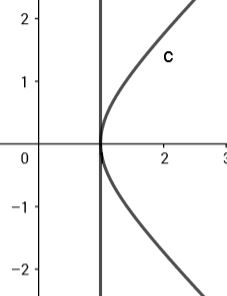
\includegraphics[scale=0.35]{ChapterCalcIII/Figures/polarpic3.jpg}
\\ }{0in}
\end{enumerate}

\AnswerKeyEntry{$\cosh{t} = 1+\frac{t^2}{2!} + \frac{t^4}{4!}+\frac{t^6}{6!} + \cdots $\newline
$\sinh{t} = t + \frac{t^3}{3!} + \frac{t^5}{5!}+ \cdots $ \newline
a.~~$\frac{d ~\sinh(t)}{dt} = 1+\frac{t^2}{2!}+\frac{t^4}{4!} + \cdots =\cosh(t)$ \newline
b.~~$\frac{d ~\cosh(t)}{dt} = t+\frac{t^3}{3!}+\frac{t^5}{5!} + \cdots =\sinh(t)$ \newline
c.~~$ \cosh^2{t}- \sinh^2{t} = \left(1+\frac{t^2}{2!} + \frac{t^4}{4!}+\frac{t^6}{6!} + \cdots \right)^2 - \left(t + \frac{t^3}{3!} + \frac{t^5}{5!}+ \cdots \right)^2 = 1 $ \newline
d.~~$\frac{1}{0}$ which is a vertical line}

\end{exercise}



\begin{exercise}{\Coffeecup \Coffeecup \Coffeecup}
\begin{enumerate}[label=\alph*.)]
\item  Graph the polar function $r(\theta)=\sin(2\theta)$.
\solushun{ \begin{tabular}{c|c}
$\theta$ & $r(\theta)$ \\ 
\hline \\
$0$ & 1 \\
$\pi/4$ & 0 \\
$\pi/2$ & -1 \\
$3\pi/4$ & 0 \\
$\pi$ &  1 \\
$5\pi/4$ & 0 \\
$3\pi/2$ & -1 \\
$7\pi/4$ & 0 \\
$2\pi$ &  1 \\
\end{tabular}
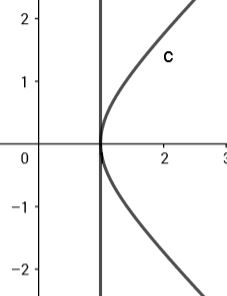
\includegraphics[scale=0.35]{ChapterCalcIII/Figures/polarpic3.jpg}
\\}{0in}
\item Find the area enclosed by one loop of that function.
\solushun{ $\int_{\frac{-\pi}{4}}^{\frac{\pi}{4}}{\frac{1}{2} (\cos{2\theta})^2~d\theta}=\frac{1}{2}\int_{\frac{-\pi}{4}}^{\frac{\pi}{4}}{\cos^2{(2\theta)}~d\theta}=\frac{1}{2} \int_{\frac{-\pi}{4}}^{\frac{\pi}{4}}{\frac{1+\cos{(4\theta)}}{2}~d\theta}= \frac{1}{4}\left(\theta + \frac{\sin{(4\theta)}}{4} \right) \Biggr|_{\frac{-\pi}{4}}^{\frac{\pi}{4}}= \frac{1}{4} \left( \frac{\pi}{4} + \frac{\sin(\pi)}{4}\right)-\frac{1}{4} \left( \frac{-\pi}{4} + \frac{\sin{(-\pi)}}{4} \right)=\frac{\pi}{16} + \frac{\pi}{16} = \frac{\pi}{8}$
\\ }{0in}
\end{enumerate}
\AnswerKeyEntry{
b.) $\frac{\pi}{8}$\newline
}
\end{exercise}

